\documentclass[pt = 12,a4paper]{article}
\usepackage{tocloft}
\renewcommand{\cftsecleader}{\cftdotfill{\cftdotsep}}
\cftsetindents{section}{0em}{4em}
\cftsetindents{subsection}{1em}{4em}
\usepackage{xcolor}
\usepackage{verbatim}
\usepackage{listings}
\usepackage{vntex}
\usepackage{a4wide,amssymb,epsfig,latexsym,array,hhline,fancyhdr}
\usepackage{enumitem}
\usepackage{MnSymbol,wasysym}
\usepackage{tikzsymbols}
\usepackage{textcomp}
\usepackage{parskip}
\usepackage[normalem]{ulem}
\usepackage{graphicx}
\usepackage[makeroom]{cancel}
\usepackage{amsmath}
\usepackage{amsthm}
\usepackage{multicol,longtable,amscd}
\usepackage{diagbox}
\usepackage{booktabs}
\usepackage{alltt}
\usepackage[framemethod=tikz]{mdframed}
\usepackage{caption,subcaption}
\usepackage{hyperref}
\usepackage{minted}
\usepackage{lastpage}
\usepackage[lined,boxed,commentsnumbered]{algorithm2e}
\usepackage{enumerate}
\usepackage{color}
\usepackage{graphicx}
\usepackage{array}
\usepackage{tabularx, caption}
\usepackage{multirow}
\usepackage{multicol}
\usepackage{rotating}
\usepackage{graphics}
\usepackage{geometry}
\usepackage{setspace}
\usepackage{epsfig}
\usepackage{tcolorbox}
\usepackage{changepage}
\renewcommand\thepart{\Alph{part}}
\renewcommand\thesection{\Roman{section}}
\renewcommand\thesubsection{\arabic{subsection}}
\usepackage{titlesec}
\titleformat*{\section}{\fontsize{20pt}{0pt}\selectfont \bfseries }
\usepackage{tikz}
\usetikzlibrary{arrows,snakes,backgrounds}
\hypersetup{colorlinks=true,linkcolor=blue}
\usepackage{hyperref}

\makeatletter
\renewcommand\tableofcontents{%
  \section*{\centering\contentsname
    \@mkboth{%
      \MakeUppercase\contentsname}{\MakeUppercase\contentsname}}%
  \@starttoc{toc}%
}
\makeatother

\setlength{\headheight}{40pt}
\pagestyle{fancy}
\fancyhead{} % clear all header fields
\fancyhead[L]{
 \begin{tabular}{rl}
    \begin{picture}(25,15)(0,0)
    \put(0,-8){
\includegraphics[width=8mm, height=8mm]{hcmut.png}}
   \end{picture}&
	\begin{tabular}{l}
		\textbf{\bf \ttfamily Trường đại học Bách Khoa thành phố Hồ Chí Minh}\\
		\textbf{\bf \ttfamily Khoa Khoa học và kĩ thuật máy tính}
	\end{tabular} 	
 \end{tabular}
}
\fancyhead[R]{
	\begin{tabular}{l}
		\tiny \bf \\
		\tiny \bf 
	\end{tabular}  }
\fancyfoot{} % clear all footer fields
\renewcommand{\headrulewidth}{0.3pt}
\renewcommand{\footrulewidth}{0.3pt}
\fancyfoot[R]{\scriptsize \ttfamily \textbf{\textcolor{red}{Trang}} {\textbf{\textcolor{red}{\thepage}}}/\pageref{LastPage}}
\renewcommand{\headrulewidth}{0.3pt}
\renewcommand{\footrulewidth}{0.3pt}
%%%
\setcounter{secnumdepth}{4}
\setcounter{tocdepth}{3}
\makeatletter
\newcounter {subsubsubsection}[subsubsection]
\renewcommand\thesubsubsubsection{\thesubsubsection .\@alph\c@subsubsubsection}
\newcommand\subsubsubsection{\@startsection{subsubsubsection}{4}{\z@}%
                                     {-3.25ex\@plus -1ex \@minus -.2ex}%
                                     {1.5ex \@plus .2ex}%
                                     {\normalfont\normalsize\bfseries}}
\newcommand*\l@subsubsubsection{\@dottedtocline{3}{10.0em}{4.1em}}
\newcommand*{\subsubsubsectionmark}[1]{}
\makeatother



\setlength{\parindent}{0pt}
\usepackage{graphicx} 
\usepackage{xcolor}
\usepackage{tikz} 
\usepackage{scrextend}
\changefontsizes{14pt}
\usetikzlibrary{calc}

\newmdenv[linecolor=black,skipabove=\topsep,skipbelow=\topsep,
leftmargin=-5pt,rightmargin=-5pt,
innerleftmargin=5pt,innerrightmargin=5pt]{mybox}
\def\thesislayout{	% A4: 210 × 297
	\geometry{
		a4paper,
		total={160mm,240mm},  % fix over page
		left=30mm,
		top=30mm,
	}
}
\lstset{
    language=R,
    basicstyle=\ttfamily\small,
    keywordstyle=\color{blue}\ttfamily,
    stringstyle=\color{black}\ttfamily,
    commentstyle=\color{green}\ttfamily,
    morecomment=[l][\color{magenta}]{\#},
    numbers=left,
    numberstyle=\tiny\color{gray},
    stepnumber=1,
    numbersep=10pt,
    backgroundcolor=\color{white},
    tabsize=4,
    showspaces=false,
    showstringspaces=false,
    breaklines=true
}
\thesislayout
\begin{document}

\begin{titlepage}
\begin{tikzpicture}[remember picture,overlay,inner sep=0,outer sep=0]
     \draw[blue!70!black,line width=4pt] ([xshift=-1.5cm,yshift=-2cm]current page.north east) coordinate (A)--([xshift=1.5cm,yshift=-2cm]current page.north west) coordinate(B)--([xshift=1.5cm,yshift=2cm]current page.south west) coordinate (C)--([xshift=-1.5cm,yshift=2cm]current page.south east) coordinate(D)--cycle;

     \draw ([yshift=0.5cm,xshift=-0.5cm]A)-- ([yshift=0.5cm,xshift=0.5cm]B)--
     ([yshift=-0.5cm,xshift=0.5cm]B) --([yshift=-0.5cm,xshift=-0.5cm]B)--([yshift=0.5cm,xshift=-0.5cm]C)--([yshift=0.5cm,xshift=0.5cm]C)--([yshift=-0.5cm,xshift=0.5cm]C)-- ([yshift=-0.5cm,xshift=-0.5cm]D)--([yshift=0.5cm,xshift=-0.5cm]D)--([yshift=0.5cm,xshift=0.5cm]D)--([yshift=-0.5cm,xshift=0.5cm]A)--([yshift=-0.5cm,xshift=-0.5cm]A)--([yshift=0.5cm,xshift=-0.5cm]A);


     \draw ([yshift=-0.3cm,xshift=0.3cm]A)-- ([yshift=-0.3cm,xshift=-0.3cm]B)--
     ([yshift=0.3cm,xshift=-0.3cm]B) --([yshift=0.3cm,xshift=0.3cm]B)--([yshift=-0.3cm,xshift=0.3cm]C)--([yshift=-0.3cm,xshift=-0.3cm]C)--([yshift=0.3cm,xshift=-0.3cm]C)-- ([yshift=0.3cm,xshift=0.3cm]D)--([yshift=-0.3cm,xshift=0.3cm]D)--([yshift=-0.3cm,xshift=-0.3cm]D)--([yshift=0.3cm,xshift=-0.3cm]A)--([yshift=0.3cm,xshift=0.3cm]A)--([yshift=-0.3cm,xshift=0.3cm]A);

   \end{tikzpicture}
\begin{center}
    \vspace{-2cm}
    \fontsize{16pt}{17pt}\selectfont 
    \textbf{\\ĐẠI HỌC QUỐC GIA TP. HỒ CHÍ MINH}
    \textbf{\\TRƯỜNG ĐẠI HỌC BÁCH KHOA}
    

\end{center}
 \vspace{10pt}
 \begin{center}
     
\includegraphics[scale=1]{hcmut.png}
 \end{center}

\begin{center}
    \fontsize{18pt}{0pt}\selectfont \textbf{BÁO CÁO} \\
\vspace{1pt}
\textbf{\fontsize{18pt}{0pt}\selectfont MÔN HỌC:Lập trình WEB }\\
\vspace{0.5cm}
\underline
{\fontsize{16pt}{1pt} \selectfont \textbf{Đề tài: }} \\
\vspace{0.5cm}
{\fontsize{14pt}{1pt} \selectfont \textbf{Khoa: Khoa Học và Kỹ Thuật Máy Tính}}
\end{center}
\vspace{0.5cm}
\centering
 \textbf{Giảng viên hướng dẫn: Nguyễn Hữu Hiếu }


\fontsize{12pt}{25pt}\selectfont
{\textbf{Danh sách thành viên:}

\begin{tabular}{|c|l|l|c|} \hline 
  \multicolumn{1}{|c|}{STT} & \multicolumn{1}{c|}{Họ và tên} & \multicolumn{1}{c|}{MSSV} & \multicolumn{1}{c|}{email} \\ \hline
  1 & Hoàng Anh Duy & 2310458 & duy.hoangtheengine@hcmut.edu.vn   \\ \hline
  2 & Đỗ Quang Long & 2311896 &  long.doquang1896@hcmut.edu.vn  \\ \hline
  3 & Lê Thuý Hiền & 2310990 & hien.lethuy@hcmut.edu.vn   \\ \hline
  4 & Đoàn Quốc Minh & 2312054 & minh.doan11102005@hcmut.edu.vn     \\ \hline
\end{tabular}}
\end{titlepage}


\newpage
\footnotesize
\tableofcontents
\thispagestyle{empty}
\addtocontents{toc}{\protect\thispagestyle{empty}}
\clearpage
\large
\newpage
\footnotesize
\phantomsection
    \vspace{-2cm}
\selectfont 

\section*{Phân công:}
\begin{tabular}{|c|l|l|c|c|}\hline
  \multicolumn{1}{|c|}{STT} & \multicolumn{1}{c|}{Họ và tên} & \multicolumn{1}{c|}{MSSV} & \multicolumn{1}{c|}{Nhiệm vụ}& Đánh giá \\ \hline
  1 & Hoàng Anh Duy & 2310458 &  &   \\ \hline
  2 & Đỗ Quang Long & 2311896 &  &  \\ \hline
  3 & Lê Thuý Hiền & 2310990 &  & \\ \hline
  4 & Đoàn Quốc Minh & 2312054 &  &  \\ \hline
\end{tabular}
\newpage
\pagenumbering{arabic}
\section{Lời mở đầu}
\hspace{0.4cm} Trong vài thập kỉ gần đây, công nghệ thông tin đã có những bước phát triển mạnh mẽ toàn diện theo cả chiều rộng và sâu. Thiết bị điện tử được sử dụng phổ biến rộng rải, len lỏi trong mọi góc của đời sống thường ngày, nó là một phần không thể thiếu trong sinh hoạt gia đình, kinh tế, công việc, xã hội... . Ứng dụng công nghệ thông tin và tin học hóa được xem là một trong những yếu tố mang tính chiến lược trong hoạt động của quốc gia, tổ chức và trong cả các cửa hàng. Nó đóng vai trò hết sức quan trọng và đã tạo nên một bước đột phá mạnh mẽ cho nhân loại. \\

\hspace{0.4cm} Mạng Internet là một trong những sản phẩm có giá trị hết sức lớn lao nó đã trở thành hạ tầng không thể thiếu, là nền tảng để truyền tải, trao đổi thông tin trên toàn cầu. Ứng dụng Internet chúng ta sẽ hoàn thành công việc với tốc độ nhanh hơn, chi phí thấp hơn nhiều so với cách thức truyền thống. Chính điều này đã thúc đẩy sự khai sinh và phát triển của thương mại điện tử trên khắp thế giới, làm biến đổi đáng kể bộ mặt văn hóa, nâng cao đời sống con người.\\

\hspace{0.4cm} Trong hoạt động sản xuất, kinh doanh, thương mại điện tử thương mại điện tử đã khẳng định được vị thế của mình và thúc đẩy sự phát triển của doanh nghiệp. Đối với các hộ kinh doanh nhỏ việc quảng bá và giới thiệu sản phẩm đến khách hàng đáp ứng nhu cầu mua sắm ngày càng cao của khách hàng sẽ rất cần thiết. Nền kinh tế ngày càng phát triển, cuộc sống của con người ngày càng được cải thiện và nâng cao, nhu cầu mua bán qua mạng ngày càng nhiều. Trong xu thế cạnh tranh ngày càng mạnh mẽ và hội nhập sâu rộng như hiện nay đòi hỏi chúng ta phải tìm ra được hướng đi tối ưu mà vẫn đạt được lợi nhuận cao. Nhóm chúng em đã lựa chọn đề tài xây dựng hệ thống bán cafe trực tuyến (Online Coffee shop) nhằm đáp ứng nhu cầu phục vụ khách hàng tiện lợi, giải quyết vấn đề khách không thể ra trực tiếp cửa hàng hoặc muốn sử dụng sản phẩm của cửa hàng tại nhà.

\newpage
\section{Phân tích bài toán}
\subsection{Giới thiệu đề tài}

\hspace{0.4cm}Sự phát triển mạnh mẽ của cuộc cách mạng công nghiệp 4.0 đã tạo ra những thay đổi sâu rộng trong nhiều lĩnh vực của đời sống, đặc biệt là trong hoạt động kinh doanh và thương mại. Công nghệ thông tin không chỉ góp phần thúc đẩy nền kinh tế phát triển mà còn làm cho cuộc sống của con người trở nên tiện lợi và hiện đại hơn. Trong bối cảnh đó, nhu cầu của người tiêu dùng không chỉ dừng lại ở việc đáp ứng các nhu cầu cơ bản mà còn hướng đến sự tiện nghi, nhanh chóng và trải nghiệm mua sắm tốt hơn.\\

\hspace{0.4cm}Đối với lĩnh vực kinh doanh cà phê, bên cạnh việc phát triển các cửa hàng truyền thống, việc mở rộng sang hình thức bán hàng trực tuyến đang trở thành xu hướng tất yếu. Khách hàng ngày nay có xu hướng tìm kiếm thông tin sản phẩm, so sánh giá cả và thực hiện mua hàng thông qua các nền tảng trực tuyến. Điều này đặt ra yêu cầu cho các cửa hàng phải xây dựng cho mình một hệ thống bán hàng online nhằm đáp ứng nhu cầu ngày càng cao của thị trường.\\

\hspace{0.4cm}Bên cạnh đó, việc quản lý hoạt động kinh doanh như sản phẩm, đơn hàng, khách hàng hay nội dung thông tin nếu thực hiện thủ công sẽ tốn nhiều thời gian, dễ xảy ra sai sót và không đảm bảo hiệu quả. Do đó, cần có một hệ thống hỗ trợ vừa phục vụ bán hàng trực tuyến, vừa giúp quản lý dữ liệu một cách khoa học và hiệu quả.\\

\hspace{0.4cm}Xuất phát từ những yêu cầu thực tiễn trên, việc xây dựng một website bán cà phê cho cửa hàng với các chức năng như hiển thị sản phẩm, tìm kiếm, đặt hàng và quản lý hệ thống là cần thiết. Với đề tài “Thiết kế website bán cà phê cho cửa hàng”, nhóm sẽ tiến hành phân tích, thiết kế và xây dựng hệ thống nhằm giải quyết các vấn đề đã đặt ra, đồng thời áp dụng các kiến thức về lập trình web trong thực tế.

\subsection{Vấn đề đặt ra trước khi xây dựng website}

\hspace{0.4cm} Trước khi tiến hành xây dựng một website, việc chuẩn bị và định hướng ban đầu là bước quan trọng nhằm đảm bảo hệ thống được phát triển đúng hướng và đạt được mục tiêu đề ra. Đây không chỉ là giai đoạn lên ý tưởng giao diện mà còn bao gồm việc xác định cấu trúc tổng thể, chức năng và cách thức vận hành của website.

\hspace{0.4cm} Trước hết, cần hình dung rõ bố cục của website, bao gồm cách tổ chức các trang và luồng tương tác của người dùng. Việc xác định trước cấu trúc giúp quá trình triển khai trở nên logic, hạn chế sai sót và tạo nền tảng cho việc phát triển các chức năng sau này.

\hspace{0.4cm} Bên cạnh đó, việc lựa chọn công nghệ phù hợp đóng vai trò then chốt. Trong phát triển web, HTML và CSS được sử dụng để xây dựng và định dạng giao diện, JavaScript hỗ trợ xử lý tương tác phía người dùng, trong khi PHP đảm nhiệm việc xử lý logic nghiệp vụ và kết nối với cơ sở dữ liệu MySQL để lưu trữ và quản lý dữ liệu. Việc tham khảo một số framework có sẵn như Bootstrap hay các thư viện có sẵn có thể tiết kiệm rất nhiều thời gian khi thiết kế website,

\hspace{0.4cm} Tuy nhiên, vấn đề không chỉ nằm ở việc sử dụng các công nghệ riêng lẻ mà còn ở cách phối hợp chúng trong một hệ thống thống nhất. Cần có sự phân tách rõ ràng giữa phần giao diện và phần xử lý dữ liệu nhằm đảm bảo tính dễ quản lý và khả năng mở rộng.

\hspace{0.4cm} Ngoài ra, các yếu tố như hiệu năng, bảo mật và khả năng mở rộng cũng cần được xem xét ngay từ đầu. Việc xử lý dữ liệu hợp lý và kiểm soát truy cập sẽ giúp hệ thống hoạt động ổn định và an toàn hơn.

\hspace{0.4cm} Tóm lại, giai đoạn chuẩn bị trước khi xây dựng website đóng vai trò nền tảng, giúp định hình toàn bộ hệ thống và tạo điều kiện thuận lợi cho quá trình phát triển và vận hành lâu dài.

\subsection{Mục tiêu chính của website}

\hspace{0.4cm} Website được xây dựng với mục tiêu chính là hỗ trợ hoạt động kinh doanh cà phê theo hình thức trực tuyến, tạo ra một kênh bán hàng hiệu quả và thuận tiện cho cả người bán và khách hàng. Thông qua hệ thống, khách hàng có thể dễ dàng tìm kiếm thông tin, lựa chọn sản phẩm và thực hiện mua hàng một cách nhanh chóng, góp phần nâng cao khả năng tiếp cận thị trường và gia tăng doanh thu.

\hspace{0.4cm} Bên cạnh đó, website còn đóng vai trò như một công cụ hỗ trợ quản lý sản phẩm. Hệ thống cho phép cập nhật, theo dõi và kiểm soát thông tin sản phẩm một cách linh hoạt, giúp đảm bảo dữ liệu luôn chính xác và đồng bộ. Việc quản lý hiệu quả danh mục sản phẩm góp phần nâng cao chất lượng vận hành và hỗ trợ hoạt động kinh doanh diễn ra ổn định.

\hspace{0.4cm} Ngoài ra, website hướng đến việc thu thập và lưu trữ dữ liệu liên quan đến hoạt động mua bán, bao gồm thông tin đơn hàng và doanh số. Các dữ liệu này có ý nghĩa quan trọng trong việc phân tích, đánh giá hiệu quả kinh doanh, từ đó hỗ trợ người quản lý đưa ra các quyết định phù hợp nhằm tối ưu hoạt động và phát triển hệ thống trong tương lai.

\hspace{0.4cm} Tóm lại, mục tiêu của website không chỉ dừng lại ở việc xây dựng một nền tảng bán hàng trực tuyến mà còn hướng đến việc hỗ trợ quản lý và khai thác dữ liệu, góp phần nâng cao hiệu quả kinh doanh một cách toàn diện.
\subsection{Đối tượng hướng đến }

\hspace{0.4cm} Website được xây dựng hướng đến hai nhóm đối tượng chính, bao gồm khách hàng và quản trị viên. Mỗi nhóm đảm nhận một vai trò khác nhau trong hệ thống, góp phần tạo nên hoạt động kinh doanh trực tuyến hiệu quả và ổn định.

\hspace{0.4cm}\textbf{Khách hàng (Customer):}đối tượng trung tâm của website. Nhóm người dùng này có nhu cầu tìm kiếm thông tin sản phẩm, tham khảo giá cả và thực hiện mua hàng trực tuyến. Việc tối ưu trải nghiệm cho khách hàng, từ giao diện hiển thị đến quy trình đặt hàng, có ý nghĩa quan trọng trong việc thu hút người dùng và gia tăng doanh thu cho cửa hàng.


\hspace{0.4cm} \textbf{Quản trị viên (Admin):}đối tượng chịu trách nhiệm quản lý và vận hành toàn bộ hệ thống. Quản trị viên có quyền kiểm soát dữ liệu, cập nhật thông tin sản phẩm, xử lý đơn hàng và giám sát hoạt động của website nhằm đảm bảo hệ thống vận hành ổn định và an toàn.

\hspace{0.4cm} Việc phân chia rõ ràng hai nhóm đối tượng giúp hệ thống đơn giản hóa trong thiết kế và triển khai, đồng thời vẫn đảm bảo đáp ứng đầy đủ các chức năng cần thiết cho hoạt động kinh doanh trực tuyến.

\section{Xác định yêu cầu bài toán:}
\subsection{Chức năng chính của hệ thống}

\hspace{0.4cm} Hệ thống website được xây dựng nhằm hỗ trợ hoạt động kinh doanh trực tuyến, bao gồm các chức năng cơ bản sau:

\hspace{0.4cm} \textbf{Quản lý sản phẩm:} Cho phép thêm, sửa, xóa và cập nhật thông tin sản phẩm. Đồng thời hỗ trợ hiển thị và giới thiệu sản phẩm đến người dùng một cách trực quan và đầy đủ.

\hspace{0.4cm} \textbf{Quản lý khách hàng:} Lưu trữ và quản lý thông tin người dùng, bao gồm đăng ký, đăng nhập, cập nhật thông tin cá nhân và theo dõi hoạt động của khách hàng trên hệ thống.

\hspace{0.4cm} \textbf{Quản lý đơn hàng:} Hỗ trợ xử lý các hoạt động liên quan đến đơn hàng như tạo đơn, cập nhật trạng thái, theo dõi quá trình xử lý và lưu trữ lịch sử giao dịch.

\hspace{0.4cm} \textbf{Quản lý bán hàng:} Đảm bảo quá trình mua bán diễn ra liên tục, từ việc khách hàng lựa chọn sản phẩm, thêm vào giỏ hàng đến hoàn tất thanh toán. Chức năng này đóng vai trò kết nối giữa người dùng và hệ thống xử lý đơn hàng.

\hspace{0.4cm} \textbf{Quản lý hệ thống:} Cho phép quản trị viên kiểm soát toàn bộ hoạt động của website, bao gồm phân quyền người dùng, quản lý dữ liệu và đảm bảo hệ thống vận hành ổn định, an toàn.

\hspace{0.4cm} Các chức năng trên được thiết kế nhằm đảm bảo hệ thống hoạt động hiệu quả, hỗ trợ tốt cho quá trình kinh doanh và mang lại trải nghiệm thuận tiện cho người dùng.

\subsection{Yêu cầu của bài toán}

\hspace{0.4cm} \textbf{Yêu cầu về công nghệ và môi trường phát triển:} Hệ thống phải được xây dựng sử dụng các công nghệ đã học bao gồm HTML5, CSS3, JavaScript, PHP và MySQL. Các xử lý phía server bắt buộc sử dụng PHP (phiên bản 7.0 trở lên) và không được sử dụng bất kỳ PHP framework, CMS hoặc CMF nào. Hệ thống có thể áp dụng mô hình MVC nhưng phải tự xây dựng. Ngoài ra, giao diện cần đảm bảo chuẩn W3C và hỗ trợ responsive design để hiển thị tốt trên nhiều thiết bị khác nhau.

\hspace{0.4cm} \textbf{Yêu cầu về các trang giao diện:} Website cần xây dựng đầy đủ các trang cơ bản bao gồm: trang chủ, trang giới thiệu, trang sản phẩm/dịch vụ, bảng giá, liên hệ, hỏi đáp và tin tức. Ngoài ra, cần có các trang chức năng như đăng ký, đăng nhập, giỏ hàng, thanh toán (nếu có) và các trang quản lý dành cho quản trị viên.

\hspace{0.4cm} \textbf{Yêu cầu về chức năng đối với khách (Guest):} Người dùng chưa đăng nhập có thể truy cập và xem các nội dung công khai trên website như sản phẩm, tin tức, thông tin liên hệ. Ngoài ra, khách có thể sử dụng chức năng tìm kiếm để tìm sản phẩm hoặc nội dung và thực hiện đăng ký, đăng nhập vào hệ thống.

\hspace{0.4cm} \textbf{Yêu cầu về chức năng đối với thành viên (User):} Sau khi đăng nhập, người dùng có thể thực hiện các thao tác như thay đổi thông tin cá nhân, mật khẩu, cập nhật hình ảnh đại diện. Ngoài ra, hệ thống cần hỗ trợ người dùng viết bình luận, đánh giá sản phẩm hoặc bài viết và sử dụng các chức năng nâng cao khác dành riêng cho thành viên.

\hspace{0.4cm} \textbf{Yêu cầu về chức năng đối với quản trị viên (Admin):} Quản trị viên có quyền quản lý toàn bộ hệ thống bao gồm quản lý người dùng (xem, sửa, khóa, xóa), quản lý bình luận và đánh giá, quản lý thông tin liên hệ từ khách hàng. Ngoài ra, quản trị viên có thể quản lý nội dung các trang public như sản phẩm, dịch vụ, bảng giá và tin tức thông qua các thao tác thêm, sửa, xóa. Hệ thống cũng cần hỗ trợ quản lý tài nguyên như hình ảnh và nội dung website.

\hspace{0.4cm} \textbf{Yêu cầu về cơ sở dữ liệu:} Hệ thống cần thiết kế cơ sở dữ liệu sử dụng MySQL để lưu trữ toàn bộ thông tin của ứng dụng, bao gồm dữ liệu người dùng, sản phẩm, đơn hàng, bài viết và các thông tin liên quan. Cơ sở dữ liệu cần đảm bảo tính nhất quán, tránh dư thừa và hỗ trợ truy vấn hiệu quả.

\hspace{0.4cm} \textbf{Yêu cầu về kiểm tra và xử lý dữ liệu:} Tất cả các dữ liệu đầu vào từ người dùng cần được kiểm tra hợp lệ ở cả phía client (JavaScript) và phía server (PHP). Hệ thống cần đảm bảo xử lý dữ liệu chính xác trước khi lưu vào cơ sở dữ liệu.

\hspace{0.4cm} \textbf{Yêu cầu về bảo mật và tối ưu:} Hệ thống cần tìm hiểu và áp dụng các biện pháp bảo mật cơ bản nhằm hạn chế các lỗ hổng như SQL Injection, XSS và truy cập trái phép. Ngoài ra, cần tìm hiểu và áp dụng các kỹ thuật SEO cơ bản để cải thiện khả năng hiển thị của website trên công cụ tìm kiếm.

\hspace{0.4cm} \textbf{Yêu cầu bổ sung:} Hệ thống cần hỗ trợ phân trang (pagination) đối với các danh sách dữ liệu lớn, hỗ trợ upload hình ảnh lên server và sử dụng các thư viện CSS/JavaScript để cải thiện giao diện và trải nghiệm người dùng.
\subsection{Yêu cầu đặt ra cho hệ thống}
\subsubsection{Yêu cầu về mặt thiết kế hệ thống:}

\hspace{0.4cm} Hệ thống được thiết kế theo mô hình client-server, trong đó phía client (trình duyệt) chịu trách nhiệm hiển thị giao diện và gửi yêu cầu, phía server (Apache kết hợp PHP) thực hiện xử lý logic và tương tác với cơ sở dữ liệu MySQL. Mô hình này giúp phân tách rõ ràng giữa các thành phần, đảm bảo tính mở rộng và dễ bảo trì.

\hspace{0.4cm} Về tổ chức mã nguồn, hệ thống được xây dựng theo hướng phân tách giữa giao diện và xử lý logic. Giao diện sử dụng HTML5, CSS3, JavaScript và framework Bootstrap để đảm bảo khả năng hiển thị và tương tác. Phần xử lý phía server sử dụng PHP để tiếp nhận request, xử lý dữ liệu và điều phối luồng hoạt động của hệ thống. Các chức năng được chia thành các module như sản phẩm, người dùng và đơn hàng nhằm giảm sự phụ thuộc giữa các thành phần và tăng khả năng bảo trì.

\hspace{0.4cm} Về thiết kế cơ sở dữ liệu, hệ thống sử dụng hệ quản trị cơ sở dữ liệu MySQL và được xây dựng dựa trên mô hình thực thể - liên kết (ERD). Việc phân chia các thực thể giúp tổ chức dữ liệu rõ ràng, phục vụ trực tiếp cho các chức năng của hệ thống.

% \hspace{0.4cm} Đối với các mối quan hệ giữa các thực thể, hệ thống sử dụng các bảng trung gian để xử lý các quan hệ nhiều-nhiều. Cụ thể, mối quan hệ giữa đơn hàng và sản phẩm được triển khai thông qua bảng \textit{order\_details}, cho phép lưu trữ thông tin chi tiết như số lượng và giá của từng sản phẩm trong một đơn hàng. Thiết kế này giúp đảm bảo tính linh hoạt và chính xác trong quá trình xử lý dữ liệu.

\hspace{0.4cm} Cơ sở dữ liệu được thiết kế theo hướng chuẩn hóa nhằm giảm thiểu dư thừa dữ liệu và đảm bảo tính nhất quán. Các bảng dữ liệu được liên kết với nhau thông qua các khóa và ràng buộc để đảm bảo tính toàn vẹn dữ liệu. Đồng thời, cấu trúc dữ liệu được tối ưu để hỗ trợ hiệu quả cho các thao tác truy vấn như tìm kiếm sản phẩm, quản lý đơn hàng và xử lý thông tin người dùng.

\hspace{0.4cm} Về giao diện người dùng, hệ thống được thiết kế theo hướng responsive, đảm bảo hiển thị tốt trên nhiều thiết bị khác nhau. Bố cục giao diện rõ ràng, dễ điều hướng, giúp người dùng thực hiện các thao tác như tìm kiếm sản phẩm, thêm vào giỏ hàng và đặt hàng một cách thuận tiện.

\hspace{0.4cm} Ngoài ra, hệ thống đảm bảo luồng xử lý dữ liệu rõ ràng từ phía client đến server, bao gồm việc tiếp nhận request, xử lý bằng PHP, truy vấn cơ sở dữ liệu MySQL và trả về response tương ứng. Việc thiết kế này giúp hệ thống hoạt động ổn định, hạn chế lỗi và đảm bảo tính nhất quán dữ liệu trong quá trình vận hành.

\subsubsection{Yêu cầu về chức năng hệ thống}

\subsubsection{Yêu cầu về chức năng hệ thống}
\hspace{0.4cm} \textbf{Chức năng đối với người xem (Guest):}
\begin{itemize}
\item Xem danh sách sản phẩm và chi tiết sản phẩm
\item Tìm kiếm và lọc sản phẩm theo danh mục hoặc từ khóa
\end{itemize}

\hspace{0.4cm} \textbf{Chức năng đối với người dùng (User):}
\begin{itemize}
\item Đăng ký, đăng nhập và đăng xuất tài khoản
\item Xem danh sách sản phẩm và chi tiết sản phẩm
\item Tìm kiếm và lọc sản phẩm theo danh mục hoặc từ khóa
\item Thêm sản phẩm vào giỏ hàng
\item Cập nhật và quản lý giỏ hàng
\item Thực hiện đặt hàng và lựa chọn phương thức thanh toán
\item Theo dõi trạng thái và lịch sử đơn hàng
\item Đánh giá và bình luận sản phẩm
\item Gửi thông tin liên hệ hoặc tin nhắn đến cửa hàng
\item Cập nhật thông tin cá nhân
\end{itemize}

\hspace{0.4cm} \textbf{Chức năng đối với quản trị viên (Admin):}
\begin{itemize}
\item Đăng nhập hệ thống quản trị
\item Quản lý sản phẩm (thêm, sửa, xóa)
\item Quản lý danh mục sản phẩm
\item Quản lý đơn hàng (xem, cập nhật trạng thái)
\item Quản lý người dùng
\item Quản lý nội dung (tin tức, bài viết)
\item Quản lý bình luận và đánh giá
\item Xử lý và phản hồi liên hệ từ khách hàng
\item Quản lý hệ thống và dữ liệu tổng thể
\end{itemize}

\section{Cơ Sở lý thuyết:}
\subsection{Ngôn ngữ đánh dấu HTML}
HTML (HyperText Markup Language) là ngôn ngữ tiêu chuẩn dùng để xây dựng cấu trúc của trang web. HTML sử dụng các thẻ (tags) để xác định các thành phần như tiêu đề, đoạn văn, hình ảnh, liên kết, bảng và biểu mẫu.

Trong hệ thống, HTML đóng vai trò:
\begin{itemize}
    \item Xây dựng cấu trúc giao diện người dùng
    \item Tổ chức nội dung theo dạng phân cấp (DOM -- Document Object Model)
    \item Là nền tảng để CSS và JavaScript tương tác và xử lý
\end{itemize}

\subsection{Ngôn ngữ định kiểu CSS}
CSS (Cascading Style Sheets) được sử dụng để định dạng và trình bày giao diện của trang web.

Vai trò chính:
\begin{itemize}
    \item Tùy chỉnh màu sắc, font chữ, kích thước, khoảng cách
    \item Thiết kế layout (Flexbox, Grid)
    \item Hỗ trợ responsive (hiển thị trên nhiều thiết bị)
    \item Tách biệt phần giao diện khỏi logic và nội dung
\end{itemize}

CSS giúp cải thiện trải nghiệm người dùng và tăng tính thẩm mỹ của hệ thống.

\subsection{Ngôn ngữ lập trình JavaScript}
JavaScript là ngôn ngữ lập trình phía client (trình duyệt), cho phép tạo ra các chức năng tương tác động.

Ứng dụng trong hệ thống:
\begin{itemize}
    \item Xử lý sự kiện (click, input, submit, \ldots)
    \item Validate dữ liệu phía client
    \item Gửi/nhận dữ liệu bất đồng bộ (AJAX, Fetch API)
    \item Cập nhật nội dung trang mà không cần reload
\end{itemize}

JavaScript giúp tăng tính tương tác và cải thiện hiệu năng ứng dụng web.

\subsection{Ngôn ngữ lập trình PHP}
PHP (Hypertext Preprocessor) là ngôn ngữ lập trình phía server, được sử dụng rộng rãi trong phát triển web.

Vai trò:
\begin{itemize}
    \item Xử lý logic nghiệp vụ
    \item Kết nối và thao tác với cơ sở dữ liệu
    \item Xử lý form (đăng nhập, đăng ký, CRUD, \ldots)
    \item Sinh nội dung HTML động
\end{itemize}

PHP thường được nhúng trực tiếp vào HTML và chạy trên server để trả về kết quả cho client.

\subsection{Hệ quản trị cơ sở dữ liệu MySQL}
MySQL là hệ quản trị cơ sở dữ liệu quan hệ (RDBMS), sử dụng ngôn ngữ SQL để quản lý dữ liệu.

Chức năng:
\begin{itemize}
    \item Lưu trữ dữ liệu hệ thống (user, sản phẩm, đơn hàng, \ldots)
    \item Truy vấn dữ liệu bằng SQL (SELECT, INSERT, UPDATE, DELETE)
    \item Đảm bảo tính toàn vẹn và nhất quán dữ liệu
    \item Hỗ trợ phân quyền và bảo mật
\end{itemize}

MySQL thường được kết hợp với PHP để xây dựng các ứng dụng web động.

% \subsection{Mối quan hệ giữa các công nghệ}
% Trong hệ thống web, các công nghệ trên phối hợp theo mô hình client--server:

% \begin{itemize}
%     \item Client (trình duyệt): HTML, CSS, JavaScript
%     \item Server: PHP
%     \item Database: MySQL
% \end{itemize}

% Luồng xử lý cơ bản:
% \begin{enumerate}
%     \item Người dùng gửi yêu cầu từ trình duyệt
%     \item JavaScript (nếu có) xử lý trước hoặc gửi request
%     \item PHP xử lý logic và truy vấn MySQL
%     \item Server trả về HTML/CSS/JS cho client
%     \item Trình duyệt hiển thị kết quả
% \end{enumerate}

\subsection{Mô tả các Thư viện và Công nghệ sử dụng}
Dựa trên kiến trúc mã nguồn thực tế, dự án không phụ thuộc vào bất kỳ PHP Framework nào (như Laravel hay CodeIgniter) mà được xây dựng hoàn toàn từ đầu (from scratch) theo mô hình MVC. Dưới đây là các công nghệ và thư viện cốt lõi được sử dụng:

\begin{itemize}
    \item \textbf{PHP 8.x (Native PHP)}: 
    \begin{itemize}
        \item \textit{Vai trò}: Ngôn ngữ kịch bản phía máy chủ đóng vai trò hạt nhân của hệ thống. Quản lý toàn bộ logic điều hướng (Router), tương tác CSDL (Model), kiểm tra quyền (Middleware) và xử lý giao diện (Controller).
        \item \textit{Ưu điểm}: Hiệu năng cao do không bị overhead bởi các framework cồng kềnh; giúp người lập trình hiểu rõ bản chất hoạt động của một quy trình request-response HTTP.
        \item \textit{Nhược điểm}: Phải tự xây dựng các thành phần nền tảng, mất nhiều thời gian và dễ phát sinh lỗi nếu kiến trúc thiết kế không vững.
        \item \textit{Lý do sử dụng}: Đáp ứng đúng yêu cầu môn học, rèn luyện kỹ năng xây dựng kiến trúc phần mềm và làm chủ mã nguồn.
    \end{itemize}

    \item \textbf{MySQL (thông qua MySQLi)}:
    \begin{itemize}
        \item \textit{Vai trò}: Hệ quản trị cơ sở dữ liệu quan hệ lưu trữ toàn bộ dữ liệu (Users, Products, Orders, FAQs). Hệ thống giao tiếp với MySQL thông qua class \texttt{Database.php} sử dụng pattern Singleton.
        \item \textit{Ưu điểm}: Nhanh, ổn định, hỗ trợ Prepared Statements giúp bảo mật truy vấn tốt. Singleton pattern giúp tiết kiệm tài nguyên (chỉ tạo 1 connection duy nhất trong 1 vòng đời request).
        \item \textit{Nhược điểm}: Cú pháp của MySQLi đôi khi dài dòng hơn PDO, và không hỗ trợ đa nền tảng CSDL (chỉ dùng riêng cho MySQL).
    \end{itemize}

    \item \textbf{HTML5, CSS3 \& Vanilla JavaScript}:
    \begin{itemize}
        \item \textit{Vai trò}: Xây dựng giao diện hiển thị khu vực người dùng (Frontend).
        \item \textit{Ưu điểm}: Giữ cho frontend cực kỳ nhẹ, tốc độ tải trang nhanh, dễ dàng tùy biến theo thiết kế riêng mà không bị gò bó bởi các class của CSS framework.
        \item \textit{Nhược điểm}: Tốn nhiều công sức để viết mã CSS cho tính năng Responsive trên các thiết bị màn hình nhỏ.
    \end{itemize}

    \item \textbf{SRTDash \& Bootstrap 5 (Khu vực Admin)}:
    \begin{itemize}
        \item \textit{Vai trò}: SRTDash là một template quản trị được tích hợp sẵn cùng framework CSS Bootstrap 5, dùng để xây dựng Admin Dashboard (\texttt{admin/layouts/main.php}).
        \item \textit{Ưu điểm}: Cung cấp sẵn hệ thống Grid system, các component (Table, Form, Modal) và giao diện trực quan, giúp phát triển module quản trị cực kỳ nhanh chóng.
        \item \textit{Nhược điểm}: Chứa nhiều file CSS/JS không sử dụng đến, làm phình to dung lượng bộ nhớ tĩnh.
        \item \textit{Lý do sử dụng}: Tính thẩm mỹ cao, phù hợp cho phân hệ quản trị yêu cầu nhiều chức năng phức tạp, giao diện bảng biểu mà không cần tốn thời gian thiết kế lại từ đầu.
    \end{itemize}

    \item \textbf{Các thư viện hỗ trợ UI/UX khác}:
    \begin{itemize}
        \item \textbf{Chart.js}: Xử lý việc vẽ các biểu đồ thống kê trực quan (biểu đồ đường, biểu đồ tròn) trên trang Dashboard của Admin.
        \item \textbf{Swiper}: Tạo các hiệu ứng trượt (carousel) mượt mà cho danh sách hình ảnh hoặc khối feedback của khách hàng.
        \item \textbf{metisMenu}: Hỗ trợ tạo thanh điều hướng (sidebar đa cấp) có khả năng gập mở linh hoạt cho quản trị viên.
        \item \textbf{FontAwesome \& Google Fonts (Plus Jakarta Sans)}: Tối ưu hóa typography và hệ thống icon, tăng tính chuyên nghiệp và hiện đại cho giao diện.
    \end{itemize}
\end{itemize}

\subsection{Phân tích Lỗ hổng Bảo mật Ứng dụng Web}
Thông qua việc phân tích trực tiếp luồng xử lý mã nguồn của dự án (luồng Authentication, CRUD Model, Middleware), tình trạng bảo mật được đánh giá như sau:

\subsubsection{Các cơ chế bảo mật đã triển khai tốt}
\begin{itemize}
    \item \textbf{Ngăn chặn SQL Injection (SQLi)}: 
    \begin{itemize}
        \item \textit{Hiện trạng xử lý}: Dự án đã vô hiệu hóa hoàn toàn rủi ro SQL Injection nhờ việc sử dụng 100\% Prepared Statements. Trong các model (ví dụ \texttt{UserModel.php}), các hàm truy vấn đều sử dụng phương thức \texttt{prepare()} và \texttt{bind\_param()} của MySQLi.
        \item \textit{Đánh giá}: Rất an toàn. Dữ liệu đầu vào bị ép kiểu và tách biệt hoàn toàn khỏi cấu trúc lệnh SQL gốc.
    \end{itemize}

    \item \textbf{Bảo mật Xác thực (Authentication \& Password Hashing)}: 
    \begin{itemize}
        \item \textit{Hiện trạng xử lý}: Lớp \texttt{AuthController.php} không lưu mật khẩu dạng plaintext. Mật khẩu được băm một chiều bằng hàm \texttt{password\_hash()} với tùy chọn \texttt{PASSWORD\_DEFAULT} (sử dụng thuật toán bcrypt mã hóa mạnh). Quá trình đăng nhập được xác minh chéo bằng \texttt{password\_verify()}.
        \item \textit{Đánh giá}: Đạt tiêu chuẩn bảo mật hiện đại. Ngay cả khi hacker đánh cắp được CSDL, mật khẩu người dùng vẫn an toàn tuyệt đối trước các cuộc tấn công Brute-force hay Rainbow Table.
    \end{itemize}

    \item \textbf{Chống Cross-Site Scripting (XSS)}: 
    \begin{itemize}
        \item \textit{Hiện trạng xử lý}: Tại khu vực render giao diện (View), hệ thống đã sử dụng hàm \texttt{htmlspecialchars(\$var, ENT\_QUOTES, 'UTF-8')} một cách nhất quán để chuyển hóa các thẻ HTML đặc biệt thành định dạng ký tự an toàn trước khi in ra màn hình.
        \item \textit{Đánh giá}: Cơ chế Output Escaping này ngăn chặn hiệu quả các kịch bản Stored XSS và Reflected XSS cơ bản.
    \end{itemize}

    \item \textbf{Phân quyền (Authorization)}: 
    \begin{itemize}
        \item \textit{Hiện trạng xử lý}: Lớp \texttt{AuthMiddleware.php} cung cấp hai phương thức \texttt{requireAdmin()} và \texttt{requireLogin()}, chặn các truy cập trái phép bằng cách kiểm tra biến \texttt{\$\_SESSION['role']}.
    \end{itemize}
\end{itemize}

\subsubsection{Các lỗ hổng tiềm ẩn, nguy cơ và cách cải thiện}
Mặc dù hệ thống đã đáp ứng tốt các tiêu chuẩn cơ bản, nhưng vẫn còn tồn tại một số điểm yếu tiềm ẩn cần khắc phục:

\begin{itemize}
    \item \textbf{Lỗ hổng Upload File (Rủi ro: Cao)}:
    \begin{itemize}
        \item \textit{Hệ thống đang xử lý thế nào}: Trong phương thức \texttt{updateProfile()} của \texttt{AdminController.php}, việc kiểm tra tính hợp lệ của file ảnh upload chỉ dựa vào việc bóc tách phần mở rộng (extension) từ tên file: \texttt{pathinfo(\$file['name'], PATHINFO\_EXTENSION)}.
        \item \textit{Nguy cơ có thể gặp}: Kẻ tấn công có thể dễ dàng bypass bước kiểm tra này bằng cách đổi tên một file mã độc PHP thành \texttt{shell.php.jpg} hoặc tinh vi hơn là chèn mã PHP vào Header của một file ảnh thật. Nếu tệp được upload, chúng có thể thực thi mã độc trên máy chủ (Remote Code Execution - RCE).
        \item \textit{Cách cải thiện}: Bắt buộc sử dụng hàm \texttt{finfo\_open(FILEINFO\_MIME\_TYPE)} để đọc chữ ký byte (Magic bytes) của tệp nhằm xác định đúng định dạng thật. Đồng thời, cấu hình server không cấp quyền thực thi (execute) cho thư mục \texttt{uploads/}.
    \end{itemize}

    \item \textbf{Cross-Site Request Forgery - CSRF (Rủi ro: Trung bình)}:
    \begin{itemize}
        \item \textit{Hệ thống đang xử lý thế nào}: Dự án hiện tại hoàn toàn vắng bóng cơ chế kiểm tra CSRF Token. Các thao tác POST (như cập nhật Profile, xóa FAQ) chỉ phụ thuộc vào việc Session có đang mở hay không.
        \item \textit{Nguy cơ có thể gặp}: Nếu một Quản trị viên đang đăng nhập hệ thống và vô tình nhấp vào một liên kết độc hại, hacker có thể mượn quyền của Quản trị viên đó để gửi các HTTP POST request ngầm (ví dụ: tạo tài khoản admin mới, xóa dữ liệu) mà nạn nhân không hề hay biết.
        \item \textit{Cách cải thiện}: Tại Base Controller, cần sinh một chuỗi hash ngẫu nhiên lưu vào \texttt{\$\_SESSION['csrf\_token']}. Ở tất cả các form HTML, chèn một thẻ \texttt{<input type="hidden" name="csrf\_token" value="...">}. Phía Server sẽ kiểm chứng sự trùng khớp của token này trước khi nhận dữ liệu.
    \end{itemize}

    \item \textbf{Session Fixation (Rủi ro: Thấp)}:
    \begin{itemize}
        \item \textit{Hệ thống đang xử lý thế nào}: Sau khi xác thực thành công trong \texttt{AuthController::handleLogin()}, hệ thống gán trực tiếp dữ liệu vào Session hiện tại mà không tái tạo Session ID mới.
        \item \textit{Nguy cơ có thể gặp}: Hacker có thể "ép" nạn nhân sử dụng một Session ID do chúng định sẵn. Khi nạn nhân đăng nhập thành công trên Session ID đó, hacker nghiễm nhiên có quyền truy cập.
        \item \textit{Cách cải thiện}: Gọi hàm \texttt{session\_regenerate\_id(true);} ngay sau bước xác thực mật khẩu hợp lệ để làm mới định danh phiên.
    \end{itemize}
\end{itemize}

\subsection{Phân tích Tối ưu hóa Công cụ Tìm kiếm (SEO)}
Đối với một Website thương mại điện tử, SEO là yếu tố then chốt. Đánh giá dựa trên mã HTML render thực tế:

\subsubsection{Ưu điểm về SEO của hệ thống}
\begin{itemize}
    \item \textbf{URL Structure (URL thân thiện)}: Nhờ bộ định tuyến lõi \texttt{Router.php} hỗ trợ biểu thức chính quy (Regex), các đường dẫn của website hiển thị ở dạng tĩnh, sạch và rõ nghĩa (ví dụ: \texttt{/gioi-thieu}, \texttt{/tin-tuc}) thay vì dùng chuỗi query string (\texttt{index.php?page=gioi-thieu}). Điều này giúp Google Bot dễ dàng thu thập dữ liệu (crawl) và người dùng dễ ghi nhớ.
    \item \textbf{Semantic HTML \& Heading Structure}: Các View Frontend như trang Giới thiệu được thiết kế chặt chẽ với cấu trúc thẻ ngữ nghĩa HTML5 (\texttt{<section>}, \texttt{<main>}, \texttt{<header>}, \texttt{<footer>}). Hệ thống thẻ Heading (\texttt{<h1>}, \texttt{<h2>}) được phân cấp hợp lý, tạo ra một dàn ý chuẩn mực cho nội dung trang.
    \item \textbf{Tối ưu thẻ Hình ảnh (Image Alt)}: Đa số các thành phần \texttt{<img>} hiển thị banner hoặc sản phẩm đều được gán thuộc tính mô tả \texttt{alt} (ví dụ: \texttt{alt="Sinh viên UniPhin Coffee"}), không chỉ hỗ trợ người dùng khiếm thị (Accessibility) mà còn cải thiện thứ hạng trên Google Images.
\end{itemize}

\subsubsection{Hạn chế và Đề xuất cải thiện SEO}
\begin{itemize}
    \item \textbf{Thiếu hụt thẻ Meta chuyên sâu}:
    \begin{itemize}
        \item \textit{Hạn chế}: Layout gốc \texttt{users/layouts/main.php} chỉ hỗ trợ khai báo thẻ \texttt{<title>}. Hiện tại đang thiếu thẻ \texttt{<meta name="description">} khiến đoạn tóm tắt hiển thị trên kết quả tìm kiếm (SERP) của Google kém thu hút. Đồng thời, website không có các thẻ Open Graph (\texttt{og:title}, \texttt{og:image}), làm giảm tỷ lệ click (CTR) khi người dùng chia sẻ liên kết lên Facebook hoặc Zalo.
        \item \textit{Đề xuất cải thiện}: Bổ sung cấu trúc dữ liệu cho mảng \texttt{\$data} trong Base Controller để nhận thêm tham số \texttt{\$metaDescription} và \texttt{\$ogImage}, từ đó in ra linh hoạt theo từng trang.
    \end{itemize}
    \item \textbf{Chưa tối ưu hóa hiệu năng tải ảnh (Performance \& Lazy Loading)}:
    \begin{itemize}
        \item \textit{Hạn chế}: Các trang sử dụng nhiều hình ảnh độ phân giải cao đang tải toàn bộ ảnh ngay lập tức khi mở trang. Việc này tạo ra nút thắt cổ chai về mạng, ảnh hưởng trực tiếp đến chỉ số LCP (Largest Contentful Paint) trong báo cáo Core Web Vitals của Google.
        \item \textit{Đề xuất cải thiện}: Thêm thuộc tính \texttt{loading="lazy"} vào các thẻ \texttt{<img>} nằm ngoài khung hình hiển thị đầu tiên (below-the-fold) để trình duyệt trì hoãn việc tải tài nguyên cho đến khi người dùng thao tác cuộn tới.
    \end{itemize}
\end{itemize}

\subsection{Kiến trúc hệ thống}
Hệ thống tuân thủ kiến trúc MVC (Model - View - Controller) truyền thống.
\begin{itemize}
    \item \textbf{Front Controller Pattern}: Mọi luồng truy cập đều bắt buộc đi qua \texttt{public/index.php}, tại đây ứng dụng khởi tạo cấu hình và phân phát request tới \texttt{Router}.
    \item \textbf{Hệ thống Routing Điều hướng}: Class \texttt{Router.php} quản lý bảng băm các đường dẫn và hỗ trợ dynamic parameters dạng Regex.
    \item \textbf{Base Controller Lõi}: Xử lý logic đóng gói biến toàn cục và xuất nội dung thông qua \texttt{ob\_start()} lồng vào các Layout có sẵn.
    \item \textbf{Models Data layer}: Tương tác trực tiếp CSDL theo từng thực thể dữ liệu cụ thể.
\end{itemize}

\subsection{Cấu trúc Source Code}
Dự án áp dụng cấu trúc thư mục tiêu chuẩn, cô lập thư mục hệ thống với môi trường Public:
\begin{itemize}
    \item \textbf{backend/app/}: Chứa logic ứng dụng (controllers, models, views, middleware).
    \item \textbf{backend/core/}: Mã nguồn nền tảng tự viết của MVC framework (Router, Database, Model, Controller).
    \item \textbf{backend/config/}: Khai báo hằng số hệ thống và cấu hình kết nối.
    \item \textbf{backend/routes/}: Định nghĩa các URL của hệ thống.
    \item \textbf{backend/public/}: Document Root, chứa \texttt{index.php} và thư mục \texttt{assets/}.
\end{itemize}
\section{Thiết kế ứng dụng}
\subsection{Xác định role và chức năng:}

\subsection{Thiết kế hệ cơ sở dữ liệu (Database):}
\subsubsection{Vẽ sơ đồ thực thể ERD:}
ERD (Entity-Relationship Diagram) là sơ đồ thực thể - liên kết, được sử dụng để mô hình hóa cấu trúc dữ liệu của hệ thống một cách trực quan. ERD biểu diễn các thực thể (Entity), thuộc tính (Attribute) và mối quan hệ (Relationship) giữa các thực thể trong cơ sở dữ liệu.

Thông qua ERD, người thiết kế có thể xác định rõ các bảng dữ liệu, khóa chính (Primary Key), khóa ngoại (Foreign Key) cũng như các ràng buộc giữa các bảng. Đây là bước quan trọng trong quá trình thiết kế cơ sở dữ liệu, giúp đảm bảo tính nhất quán, tránh dư thừa dữ liệu và hỗ trợ triển khai hệ thống một cách hiệu quả.

\newpage
\textbf{Sơ đồ thực thể của website}
\begin{figure}[H]
    \centering
    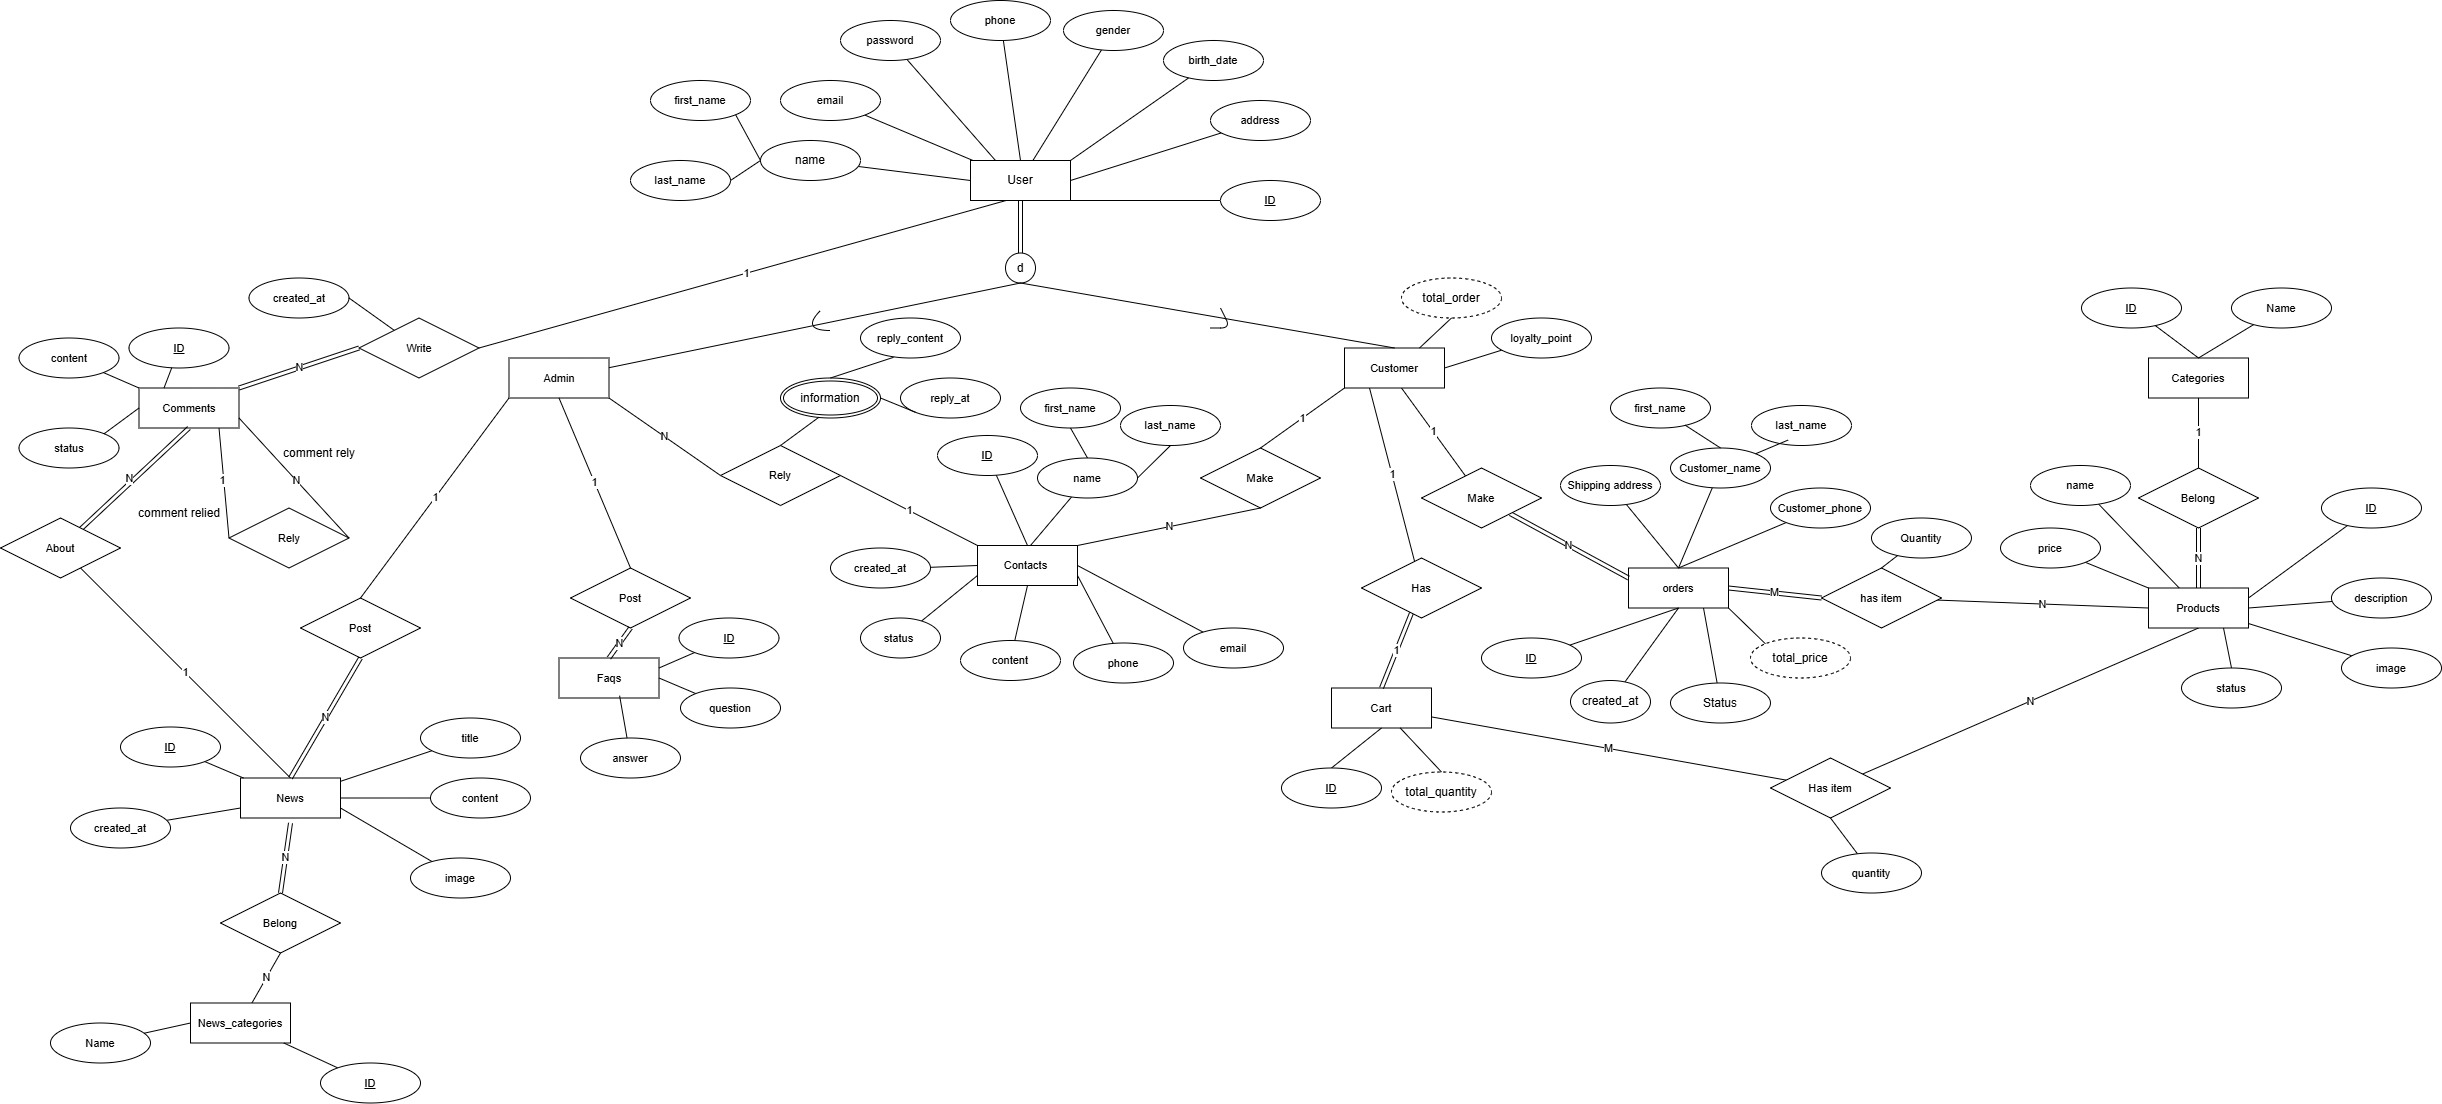
\includegraphics[width=1\linewidth]{ERD.png}
    \caption{Coffee online shop ERD}
    \label{fig:placeholder}
\end{figure}
\href{https://app.diagrams.net/#G15bkcGnWgMzCtszXc4CKO0EQjmWReY_Nt#%7B%22pageId%22%3A%2265gJjkLBR6Q1eBLMOc3a%22%7D}{Xem sơ đồ thực thể ERD tại link này}



\end{document}
